\documentclass[11pt, aspectratio=169, xcolor=table]{beamer}
\usepackage[utf8]{inputenc}
\usepackage[T1]{fontenc}
\usepackage{graphicx}
\usepackage{hyperref}
\usepackage{lmodern}
\usepackage[spanish]{babel}
\usepackage{pdfrender}
\usepackage{xcolor}
\usepackage{ragged2e}
\usepackage[version=4]{mhchem}
\usepackage{siunitx}
\renewcommand{\raggedright}{\justifying}
\usepackage{smartdiagram}
\usetheme{Berlin}

\author{Prof. Daniel Muñoz \\
	\texttt{daniel.munoz3@mail.udp.cl}
}
\title{Química Unidad 3}
\subtitle{Del caos molecular a sistemas en equilibrio}
\titlegraphic{\includegraphics[width=4cm]{../img/udplogo}}

\begin{document}

\maketitle

\section[TCM: PVNT]{Teoría cinético molecular y variables de estado}
\begin{frame}[allowdisplaybreaks]
	\frametitle{Ludwing Boltzman: 1844 - 1906}
	\begin{columns}
		\begin{column}{.5\textwidth}
			\begin{itemize}
				\scriptsize
				\item Físico Austriaco padre de la mecánica estadística.
				\item Desarrolló el concepto actualmente usado de entropía.
				\item Logró vincular propiedades macroscópicas con microscópicas mediante tratamientos estadísticos.
				\item Sus trabajos fueron continuados posteriormente por Einstein y defendidos por Planck.
				\item En 1906 se suicida, según mencionan, por falta de reconocimiento.
			\end{itemize}
		\end{column}

		\begin{column}{.5\textwidth}
			\begin{figure}[ht]
				\centering
				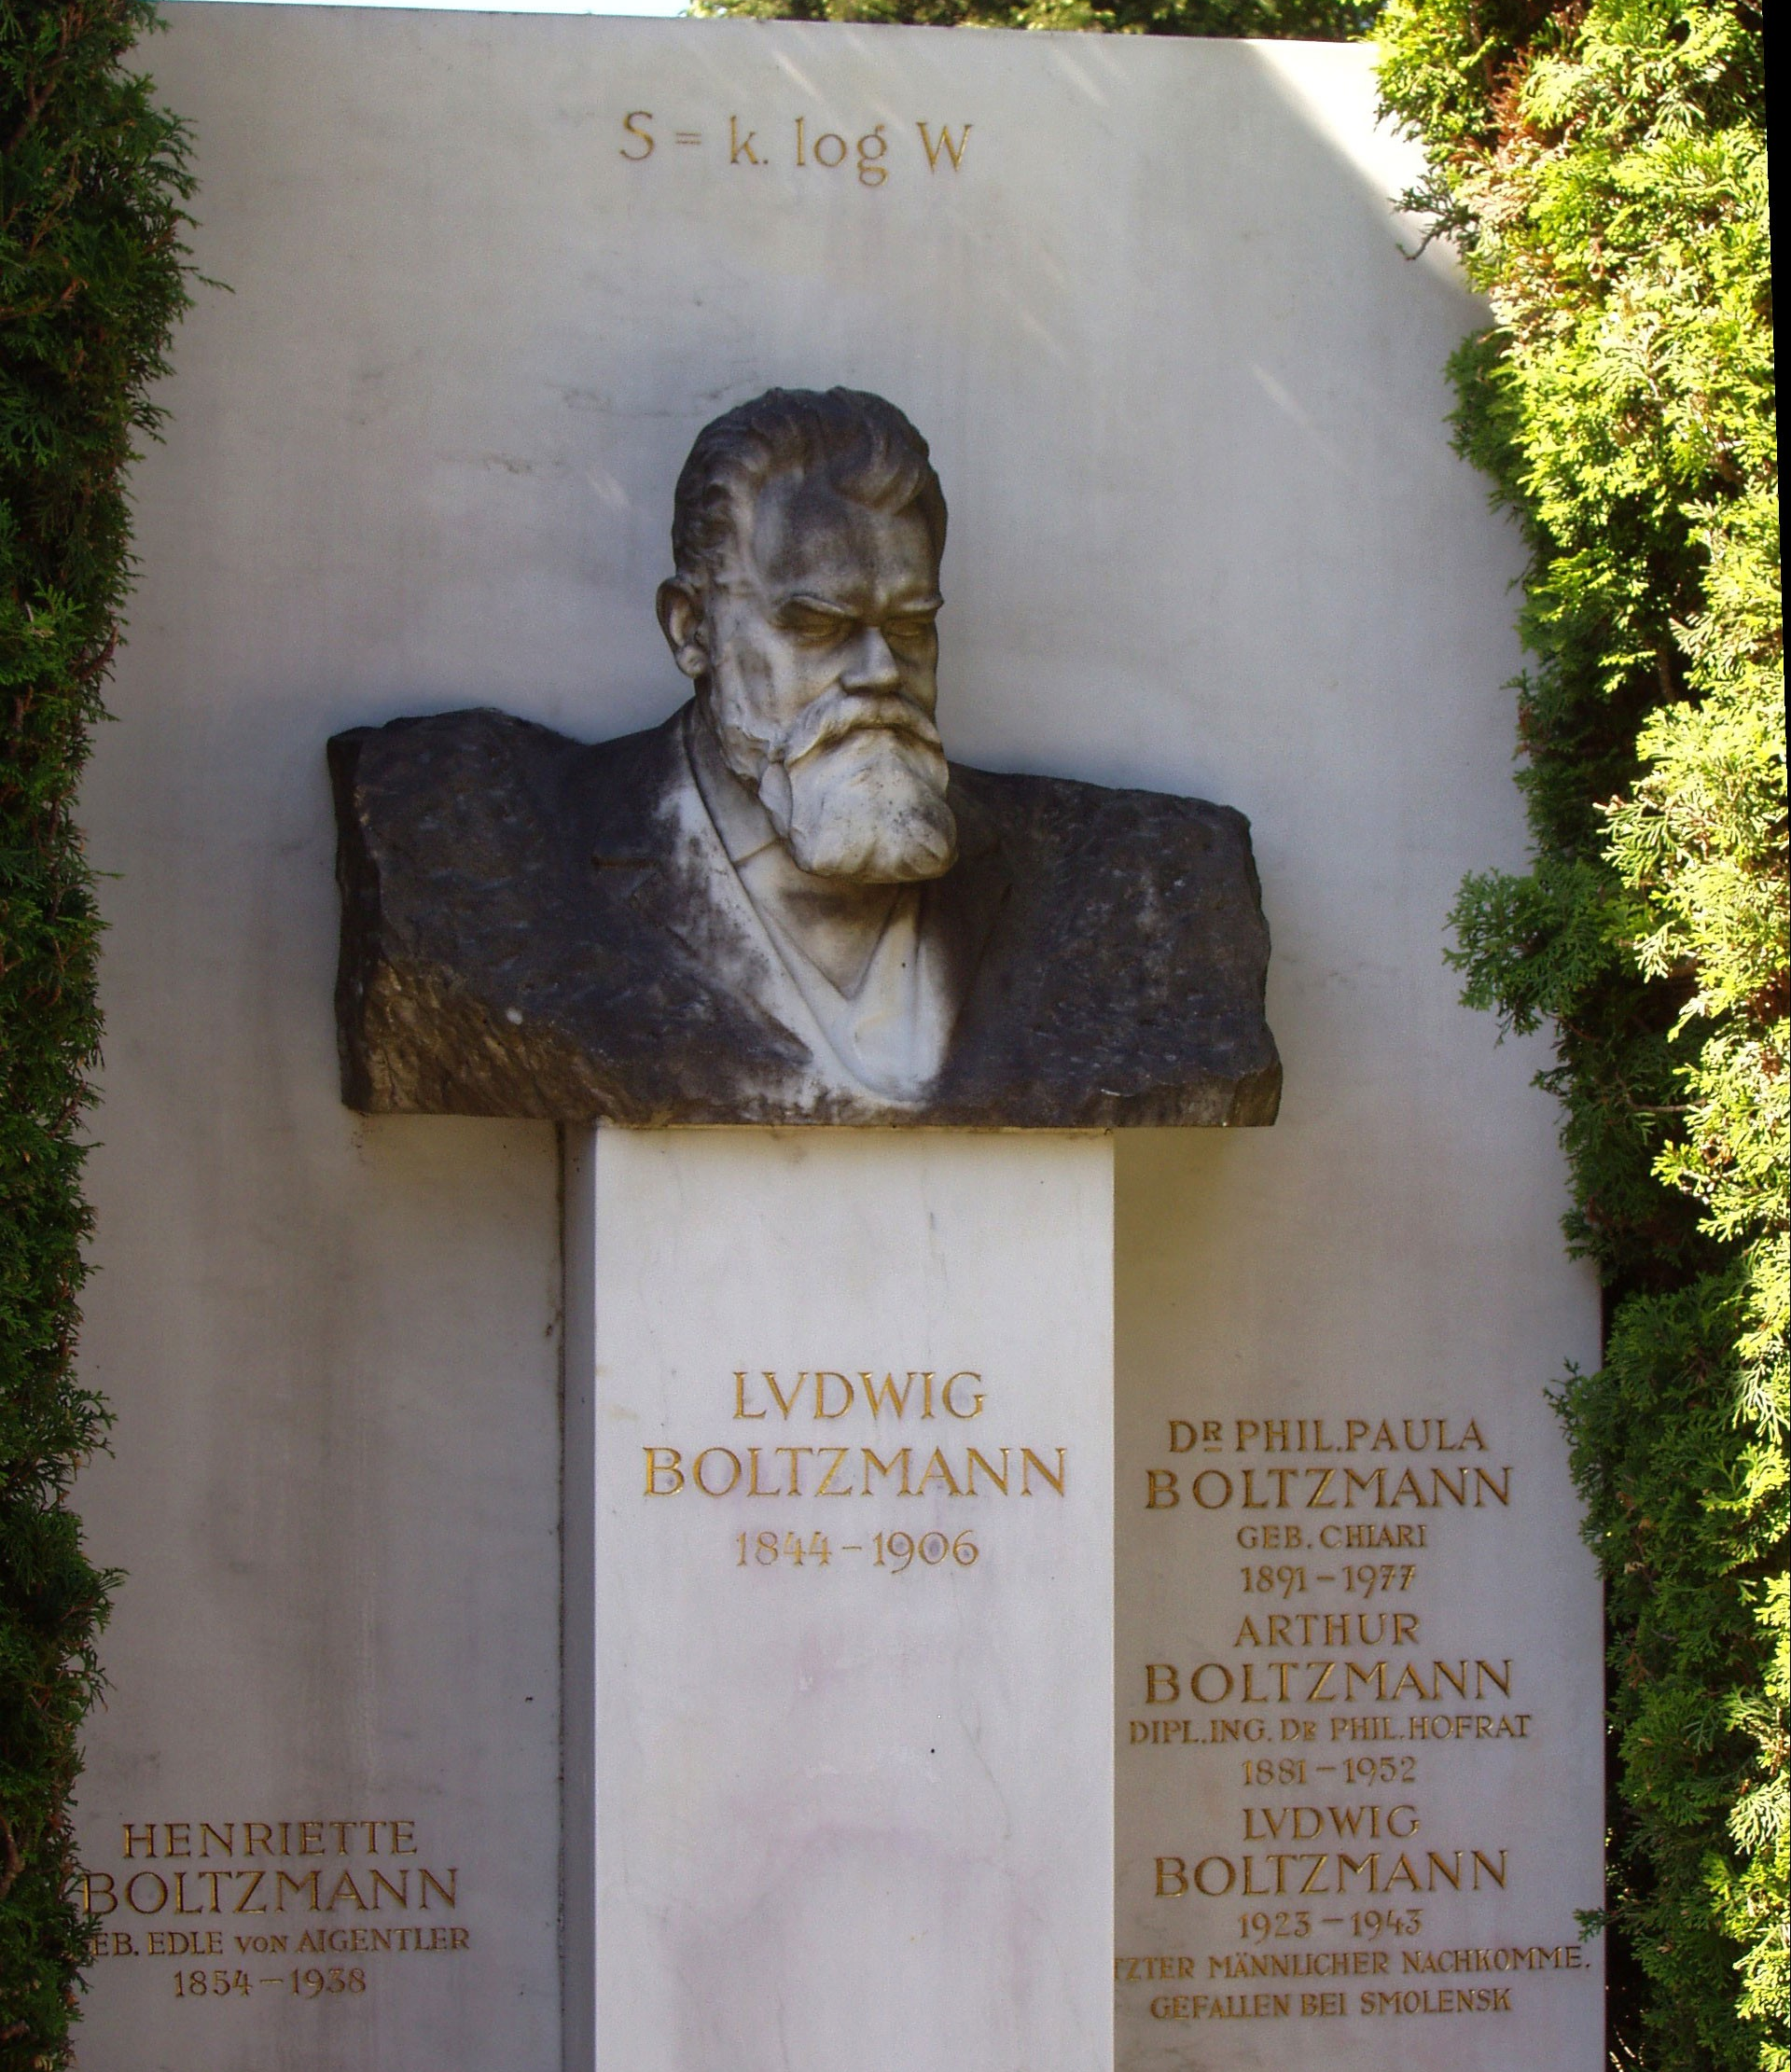
\includegraphics[height=0.6\textheight]{../img/boltzman.png}
				\caption{\label{fig:label} Tumba de Boltzman en Viena}
			\end{figure}

		\end{column}
	\end{columns}
\end{frame}

\begin{frame}
  \frametitle{Teoría Cinético Molecular (TCM)}
  \begin{columns}
    \begin{column}{0.5\textwidth}
      \begin{itemize}
        \footnotesize
        \item Una de las grandes conclusiones de LB es que para predecir el comportamiento de un gas podemos asumir que no poseen estructura interna. 
        \item Esto significa que podemos suponer el mismo comportamiento para un gas monoatómico, que para un gas poliatómico
        \item Esta sencilla, pero poderosa observación nos permite predecir un gas conocimiento muy pocos elementos de él.
        \item Actualmente sabemos que eso es cierto bajo ciertas condiciones P $\approx$ \qty{1}{atm} y T < \qty{30}{\degreeCelsius}
      \end{itemize}
    \end{column}
    \begin{column}{0.5\textwidth}
      \begin{figure}[ht]
        \centering
        \includegraphics[width=\textwidth]{../img/billar.jpg}
        \caption{El billar es un ejemplo de como se comporta microscópicamente todo gas ``ideal''}
        \label{fig:2}
      \end{figure}
    \end{column}
  \end{columns}
\end{frame}

\begin{frame}
  \frametitle{Variables de estado}
  \begin{columns}
    \begin{column}{0.5\textwidth}
      \begin{block}{Variable}
        Magnitud física que cambia. Ejemplo: tiempo.
        \begin{equation}
          \label{eq:1}
          f(x) \rightarrow x
        \end{equation}
      \end{block}
    \end{column}
    \begin{column}{0.5\textwidth}
      \begin{block}{Estado}
        Todas las variables que describen un sistema (gas).
        \begin{equation}
          \label{eq:2}
          E_{gas} = {r_1, r_2, r_3, r_3 ... r_n}
        \end{equation}
      \end{block}
    \end{column}
  \end{columns}
\end{frame}

\begin{frame}
  \frametitle{Variables y Unidades}
  \begin{columns}
    \begin{column}{0.5\textwidth}
      Las Variables que describen un gas ``ideal'' son:
      \begin{itemize}[<+->]
        \footnotesize
        \item Presión (P):Fuerza ejercida por unidad de área, sus unidades son: \unit{atm}, \unit{mmHg} o \unit{\pascal} (SI).
        \item Volumne (V): Espacio que ocupa un cuerpo (gas), sus unidades son: \unit{\liter} o \unit{\cubic\meter} (SI).
        \item Temperatura (T): Movimiento promedio de las partículas de un gas, sus unidades son: \unit{degreeCelsius}, \unit{\kelvin} (SI)
        \item Número de partículas (n), su unidad de medida es \unit{\mole} (SI)
      \end{itemize}
    \end{column}
    \begin{column}{0.5\textwidth}
      \begin{figure}[ht]
        \includegraphics<1>[width=\textwidth]{../img/presion.png}
        \only<1>{\caption{Presión}}
        \includegraphics<2>[width=\textwidth]{../img/volumen.png}
        \only<2>{\caption{Volumen}}
        \includegraphics<3>[height=0.6\textheight]{../img/temperature.jpg}
        \only<3>{\caption{Temperatura}}
        \includegraphics<4>[height=0.6\textheight]{../img/mole.jpg}
        \only<4>{\caption{Mol}}
      \end{figure}
    \end{column}
  \end{columns}
\end{frame}

\begin{frame}
  \frametitle{Sistema Internacional de Unidades (SI)}
  \begin{columns}
    \begin{column}{0.5\textwidth}
      \begin{itemize}
        \footnotesize
        \item Antiguamente para medir lo mismo se utilizaban diferentes medidas (ejemplo distancia: centimetros, codos, pulgadas, etc)
        \item Durante la revolución francesa se impuso la estandarización de medidas impulsando el sistema métrico por sobre otros.
        \item Actualmente es comúnmente aceptado usar las mismas unidades de medidas para las mismas magnitudes, existiendo dos grandes sistemas, el internacional (sistema métrico-decimal) y el anglosajón.
      \end{itemize}
    \end{column}
    \begin{column}{0.5\textwidth}
      \begin{figure}[ht]
        \includegraphics[width=0.6\textwidth]{../img/siu.png}
        \caption{Sistema Internacional de Unidades}
      \end{figure}
    \end{column}
  \end{columns}
\end{frame}

\section[Leyes de los gases]{Leyes de los gases: Boyle, Charles, Gay-Lussac y Avogadro}
\begin{frame}[allowdisplaybrakes]
  \frametitle{Ley de Boyle-Mariotte}
  \begin{columns}
    \begin{column}{0.5\textwidth}
      \begin{block}{}
        El británico-irlandés Robert Boyle (1627 - 1691) y el frances Edme Mariotte (1620 - 1684) en la década de 1670 descubren independientemente que el producto de la presión (P) por volumen (V) en un gas es constante, o dicho de otro modo, son inversamente proporcionales, cuando la temperatura (T) y la cantidad de gas (n) son constantes.
        \begin{equation}
          \label{eq:3}
          P \propto \frac{1}{V}; T,n = cte
        \end{equation}
      \end{block}
    \end{column}
    \begin{column}{0.5\textwidth}
    \begin{figure}[ht]
      \includegraphics<1>[width=0.6\textwidth]{../img/boylemariotte.png}
      \only<1>{\caption{Robert Boyle y Edme Mariotte}}
      \includegraphics<2>[width=0.6\textwidth]{../img/boyle_law.png}
      \only<2>{\caption{Datos que muestran la relación inversa $k = PV$}}
    \end{figure}
    \end{column}
  \end{columns}

\end{frame}

\begin{frame}
  \frametitle{Ley de Charles}
  \begin{columns}
    \begin{column}{0.5\textwidth}
      \begin{definition}
        Jacques Charles, químico francés en la década de 1780 descubre que para un gas el volumen (V) y la temperatura (T) del gas son directamente proporcionales, cuando la presión (P) y la cantidad de un gas (n) son constantes.
        \begin{equation}
          \label{eq:4}
          V \propto T; P,n = cte.
        \end{equation}
      \end{definition}
    \end{column}
    \begin{column}{0.5\textwidth}
      \begin{figure}[ht]
        \includegraphics<1>[width=0.5\textwidth]{../img/charles.jpg}
        \only<1>{\caption{Jacques Charles (1746 - 1823)}}
        \includegraphics<2>[width=\textwidth]{../img/charles_law.png}
        \only<2>{\caption{gráfico V y T}}
      \end{figure}
    \end{column}
  \end{columns}
\end{frame}

\begin{frame}
  \frametitle{Ley Gay-Lussac}
  \begin{columns}
    \begin{column}{0.5\textwidth}
      \begin{definition}
        Joseph-Luis Gay-Lussac fue un químico francés que en la decada de 1808 cita los trabajos de Charles y una nueva proporcionalidad, dónde la presión (P) y la temperatura (T) son proporcionales cuando el volumen (V) y la cantidad de gas (n) son constantes:
        \begin{equation}
          \label{eq:5}
          P \propto T; V,n = cte.
        \end{equation}
      \end{definition}
    \end{column}
    \begin{column}{0.5\textwidth}
      \begin{figure}[ht]
        \includegraphics<1>[width=0.5\textwidth]{../img/gaylussac.jpg}
        \only<1>{\caption{Joseph-Luis Gay-Lussac (1778 - 1850)}}
        \includegraphics<2>[width=0.6\textwidth]{../img/gaylussac_law.png}
        \only<2>{\caption{Gráfico de la Ley}}
      \end{figure}
    \end{column}
  \end{columns}
  
\end{frame}

\begin{frame}
  \frametitle{Ley de Avogadro}
  \begin{columns}
    \begin{column}{0.5\textwidth}
      \begin{definition}
        Amadeo Avogrado científico y abogado italiano descubre en 1811 que el volumen (V) y la cantidad de gas (n) son proporcionales cuando la presión (P) y la temperatura (T) son constantes.
        \begin{equation}
          \label{eq:6}
          V \propto n; P,T = cte.
        \end{equation}
      \end{definition}
    \end{column}
    \begin{column}{0.5\textwidth}
      \begin{figure}[ht]
        \includegraphics<1>[width=0.6\textwidth]{../img/avogadro.jpg}
        \only<1>{\caption{Amadeo Avogrado (1776 - 1856)}}
        \includegraphics<2>[width=0.6\textwidth]{../img/avogadro_law.png}
        \only<2>{\caption{Gráfico de la ley}}
      \end{figure}
    \end{column}
  \end{columns}
\end{frame}


\section{Aplicación de la Ley de los gases ideales}

\section{Cálculos estequimétricos en gases ideales}

\begin{frame}
  \frametitle{Bibliografía}
  \begin{thebibliography}{99}
    \setbeamertemplate{bibliography item}[book]
    \bibitem[Chang, 2011]{Chang2011}
    Chang, Raymond
    \newblock \emph{Fundamentos de Química}
    \newblock McGraw Hill, 2011
  \end{thebibliography}
\end{frame}

\end{document}
